\section{Tree-Based Data Structures} 

\subsection{Binary Trees} 

  Let us compare the HashSet/Map and the TreeSet/Map. The purpose of Hashing is to "find" and add elements quickly. 
  \begin{enumerate}
      \item This means that add, contains, put, and get are all amortized $O(1)$ (under Simple Uniform Hashing Assumption). The TreeSet/Map have all operations add, contains, put, get are $O(\log(N))$, which is slower, but is not amortized. 
      \item Trees are sorted, while Hashes are not, and so we can get a range of Tree values in sorted order efficiently, but not for Hashes. 
  \end{enumerate}

  A Node for trees is represented with the following class. 
  \begin{lstlisting}
  public class TreeNode {
      TreeNode left; 
      TreeNode right; 
      String info; 
      
      TreeNode (String s) {
          info = s; 
      }
      
      TreeNode(String s, TreeNode llink, TreeNode rlink) {
          info = s; 
          left = llink; 
          right = rlink; 
      }
  }
  \end{lstlisting}

  A tree looks pictorially like this: 
  \begin{center}
  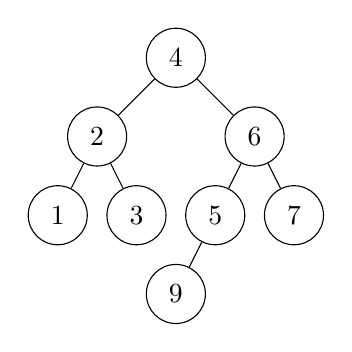
\begin{tikzpicture}[  every node/.style={    circle,    minimum size=0.75cm,    draw,    text centered,    anchor=center  }]
    \node (4) at (0,0) {4};
    \node (2) at (-1,-1) {2};
    \node (6) at (1,-1) {6};
    \node (1) at (-1.5,-2) {1};
    \node (3) at (-0.5,-2) {3};
    \node (5) at (0.5,-2) {5};
    \node (7) at (1.5,-2) {7};
    \node (9) at (0, -3) {9}; 
    \draw (4) -- (2);
    \draw (4) -- (6);
    \draw (2) -- (1);
    \draw (2) -- (3);
    \draw (6) -- (5);
    \draw (6) -- (7); 
    \draw (5) -- (9); 
  \end{tikzpicture}
  \end{center}
  Some terms: 
  \begin{enumerate}
      \item The root of the tree is the top node, which is $4$
      \item The leaf of the tree are nodes that do not have a left nor right subchild. 
      \item A path is any path from one node to another node. A simple path is a path that doesn't cross the same edge twice 
      \item The height of a node is the length of the longest downward path to a leaf from that node. 
      \item The depth of a node is the number of edges from the root to the node. 
  \end{enumerate}

  \begin{theorem}[Print All Nodes in A Binary Tree]
    Here are three ways to recursively traverse a tree. The difference is in where the nonrecursive part is. Let us have a binary tree from above. 
    \begin{enumerate}
      \item This tells us to print everything on the left of the node, then print the node, and then print everything on the right. 
      \begin{lstlisting}
      void inOrder(TreeNode t) {
          if (t != null) {
              inOrder(t.left);
              System.out.println(t.info); 
              inOrder(t.right); 
          }
      }
      // 1, 2, 3, 4, 9, 5, 6, 7
      \end{lstlisting}
      
      \item This tells us to print the node itself first, then print all the ones on the left, and then print all the ones on the right. 
      \begin{lstlisting}
      void preOrder(TreeNode t) {
          if (t != null) {
              System.out.println(t.info); 
              preOrder(t.left); 
              preOrder(t.right); 
          }
      }
      // 4, 2, 1, 3, 6, 5, 9, 7
      \end{lstlisting}
      
      \item This tells us to print all the nodes on the left, then all ones on the right, and then the node itself. 
      \begin{lstlisting}
      void postOrder(TreeNode t) {
          if (t != null) {
              postOrder(t.left); 
              postOrder(t.right); 
              System.out.println(t.info); 
          }
      }
      // 1, 3, 2, 9, 5, 7, 6
      \end{lstlisting}
    \end{enumerate}
  \end{theorem}

  \begin{theorem}[Storing All Nodes in a List]
    Now if we want to store them all in a list, then this recursive strategy will not work, since if we create a list inside the function body, then we will have a bunch of lists floating around in memory. Therefore, we want to initialize a list outside of the entire function, and store that entire thing within a wrapper function. The $\texttt{inOrder}$ takes in also a reference to a list that it will be adding to. 
    \begin{lstlisting}
      public ArrayList<String> visit(TreeNode root) {
          ArrayList<String> list = new ArrayList<>(); 
          inOrder(root, list); 
          return list; 
      }

      private void inOrder(TreeNode root, ArrayList<String> list) {
          if (root != null) {
              inOrder(root.left, list); 
              list.add(root.info); 
              inOrder(root.right, list); 
          }
      }
    \end{lstlisting}
  \end{theorem}

  \begin{definition}[Finding Height of Node]
    The height of a node is the longest downward path to a leaf from that node, so its height would be the maximum of the two heights of its children. A null node would have height $-1$, which is our base case. 
    \begin{lstlisting}
      public int getHeight(TreeNode root) {
          if (root == null) { return -1; }
          return 1 + Math.max(getHeight(root.left), getHeight(root.right)); 
      }
    \end{lstlisting}
  \end{definition}

  \begin{definition}[Finding Depth of Node]
    The depth is quite hard to find recursively, but if we have a reference to the parent, then we can write 
    \begin{lstlisting}
      int depth(TreeNode node) {
          if (node == null) {
              return -1;
          } else {
              return 1 + depth(node.parent);
          }
      }
    \end{lstlisting}
  \end{definition}

\subsection{Heaps}

  \begin{definition}[Binary Heap]
  A \textbf{binary heap} is a binary tree satisfying the following structural invariants: 
  \begin{enumerate}
      \item Maintain the \textbf{heap property} that every node is less than or equal to its successors, and 
      \item The \textbf{shape property} that the tree is complete (full except perhaps last level, in which case it should be filled from left to right. 
  \end{enumerate}
  We should conceptually think of a binary heap as an underlying binary heap, but it is actually usually implemented with an array, and we can create a map from the heap to the array with the following indices. 
  \begin{center}
      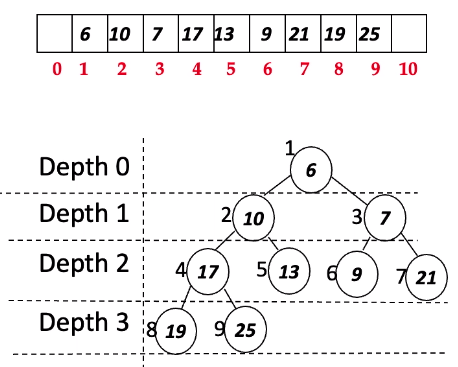
\includegraphics[scale=0.5]{img/binary_heap.png}
  \end{center}
  When 1-indexing, for node with index $k$, the left child is index $2k$, the right child is index $2k + 1$, and the parent is index $k/2$ (where this is integer division). 
  \end{definition}

  Implementing peek is easy, since we just return the first index, but it can be quite tricky to maintain this invariant after an arbitrary sequence of add/remove operations. 
  \begin{enumerate}
      \item To add values to a heap, we add to the first open position in the last level of the tree (to maintain the shape property), and then swap with the parent is the heap property is violated. If we are swapping with the parent at most $\log(N)$ times, then the add property has $O(\log(N))$ complexity. 
      \begin{center}
          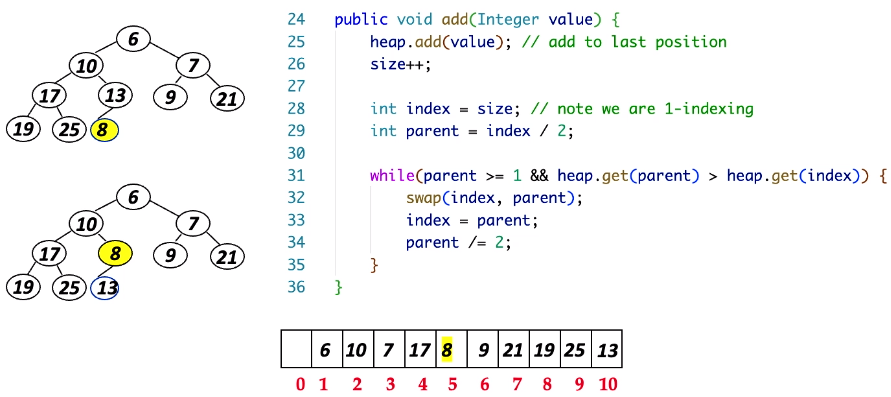
\includegraphics[scale=0.5]{img/heap_add_implementation.png}
      \end{center}
      
      \item We remove the first (minimal) value, we first replace the root with the last node in the heap, and while the heap property is violated, we swap with the smaller child. There are two choices, the left or right child, in which we can swap. But we must always swap with the \textbf{smaller child}, since we swapped with the bigger child, then this bigger child would be larger than the smaller one, violating the heap property. Since a complete binary tree always has height $O(\log(N))$, remove also "traverses" one root-leaf path, and so its runtime complexity is $O(\log(N))$, too. 
      \begin{center}
          % \includegraphics[scale=0.5]{}
      \end{center}
      
      \item The decreaseKey operation just takes an arbitrary node and decreases its value to some other integer. In this case, it wouldn't violate the shape property, and to restore the heap property, we just put swap it with its parent if the new value is smaller than its parent, making this operation $O(\log(N))$. 
  \end{enumerate}

  \begin{definition}[Priority Queues]
    A priority queue simply adds things according to their priority. Every time we add an element, it looks at where the element should go to keep the list sorted. If we want to dequeue, then we just remove the first element of the list. 
    \begin{enumerate}
      \item $\texttt{pq.add(Object element)}$ is $O(\log(N))$
      \item $\texttt{pq.remove()}$ is $O(\log(N))$ 
      \item $\texttt{pq.peek()}$ returns the minimal element and is $O(1)$
      \item $\texttt{pq.size()}$ returns number of elements and is $O(1)$
    \end{enumerate}
  \end{definition}

\subsection{Binary Search Trees}

  \begin{definition}[Binary Search Tree]
    A binary tree is a \textbf{binary search tree} if for every node, the left subtree values are all less than the node's value, and the right subtree values are all greater than the node's value. That is, the nodes are in order, and if we called $\texttt{inOrder(root)}$ on the tree, then we would get a sorted list, which allows for efficient search. 
  \end{definition}

  Adding elements to a binary search tree is also very similar. But note that the order in which we add elements to the binary search tree will matter, since it can either make the tree \textbf{balanced} or \textbf{unbalanced}. 

  \begin{figure}[H]
    \centering 
    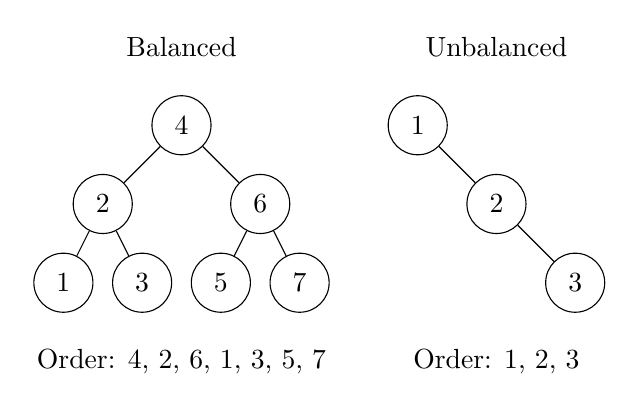
\begin{tikzpicture}[ integer/.style={    draw,    circle,    minimum size=0.75cm,    inner sep=0pt,    text centered,    anchor=center  }]
      % Balanced tree
      \node[integer] (4) at (0,0) {4};
      \node[integer] (2) at (-1,-1) {2};
      \node[integer] (6) at (1,-1) {6};
      \node[integer] (1) at (-1.5,-2) {1};
      \node[integer] (3) at (-0.5,-2) {3};
      \node[integer] (5) at (0.5,-2) {5};
      \node[integer] (7) at (1.5,-2) {7};
      \draw (4) -- (2);
      \draw (4) -- (6);
      \draw (2) -- (1);
      \draw (2) -- (3);
      \draw (6) -- (5);
      \draw (6) -- (7);

      % Caption for balanced tree
      \node at (0,1) {Balanced};
      \node at (0,-3) {Order: 4, 2, 6, 1, 3, 5, 7};

      % Unbalanced tree
      \node[integer] (1') at (3,0) {1};
      \node[integer] (2') at (4,-1) {2};
      \node[integer] (3') at (5,-2) {3};
      \draw (1') -- (2');
      \draw (2') -- (3');

      % Caption for unbalanced tree
      \node at (4,1) {Unbalanced};
      \node at (4,-3) {Order: 1, 2, 3};
    \end{tikzpicture}
    \caption{Comparison of balanced and unbalanced binary trees. In a balanced case, contains/add will be $O(\log(N))$, while in an unbalanced case, we will have $O(N)$.}
    \label{fig:trees}
  \end{figure}

  \begin{definition}[Binary Search]
    Given that we have a sorted list (this is important!), we can search for the index of an element in $O(\log{n})$ time. We want the loop invariant "if the target is in the array/list, it is in the range [low, high]." Let us have a list of $N$ elements, and at every step, we either 
    \begin{enumerate}
      \item get our desired element and its index, or 
      \item cut down our search space by half
    \end{enumerate}
  \end{definition}

  Now, we have learned how we can implement a priority queue using a binary heap. This is also possible to use a binary search tree, since it's easy to get the minimal element for adding and removing, but there are three things that make it difficult: 
  \begin{enumerate}
      \item all elements must be unique 
      \item it is not array-based, and so uses more memory and higher constant factors on runtime 
      \item it is much harder to implement with guarantees that the tree will be balanced. This makes it difficult since if we want to search through a balanced BST, it is $O(\log(N))$, but if it turns out to be unbalanced, then it is $O(N)$. 
  \end{enumerate}
  Therefore, while a balanced tree may be efficient on average, in the worst case the linear complexity is not tolerable. Therefore, we must implement a binary search tree that will do extra work to ensure that they are approximately balanced. This is where \textit{red-black trees}, which are a special type of binary search trees, come in.  

  \begin{definition}[Red-Black Tree]
    \textbf{Red-Black Trees} are binary search trees consisting of nodes that are labeled either red or black that satisfy the following properties: 
    \begin{enumerate}
      \item The root is black 
      \item A red node cannot have red children 
      \item From any node, all paths to null descendants must have the same number of black nodes. (Null is considered to be a black node)
    \end{enumerate}

    \begin{figure}[H]
      \centering
      \begin{subfigure}[b]{0.32\textwidth}
      \centering
        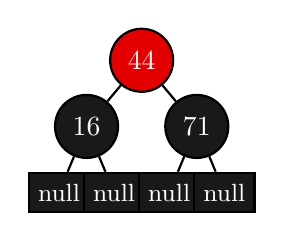
\begin{tikzpicture}[
          scale=0.7,
          red_node/.style={circle, draw, thick, fill=red!90!black, text=white, minimum size=0.8cm},
          black_node/.style={circle, draw, thick, fill=black!90, text=white, minimum size=0.8cm},
          null_node/.style={rectangle, draw, thick, fill=black!90, text=white, minimum size=0.5cm, font=\small},
          edge/.style={draw, thick, -}
        ]
        % First tree (invalid red-black tree)
        % Nodes
        \node[red_node] (n44) at (0,0) {44};
        \node[black_node] (n16) at (-1,-1.2) {16};
        \node[black_node] (n71) at (1,-1.2) {71};
        \node[null_node] (n16l) at (-1.5,-2.4) {null};
        \node[null_node] (n16r) at (-0.5,-2.4) {null};
        \node[null_node] (n71l) at (0.5,-2.4) {null};
        \node[null_node] (n71r) at (1.5,-2.4) {null};
        
        % Edges
        \draw[edge] (n44) -- (n16);
        \draw[edge] (n44) -- (n71);
        \draw[edge] (n16) -- (n16l);
        \draw[edge] (n16) -- (n16r);
        \draw[edge] (n71) -- (n71l);
        \draw[edge] (n71) -- (n71r);
        \end{tikzpicture}
        \caption{Invalid: Root node is red, violating the property that the root must be black.}
        \label{fig:rb-invalid1}
      \end{subfigure}
      \hfill 
      \begin{subfigure}[b]{0.32\textwidth}
      \centering
        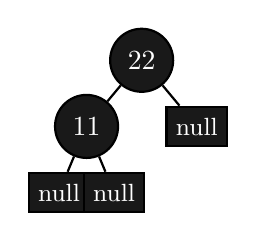
\begin{tikzpicture}[
          scale=0.7,
          red_node/.style={circle, draw, thick, fill=red!90!black, text=white, minimum size=0.8cm},
          black_node/.style={circle, draw, thick, fill=black!90, text=white, minimum size=0.8cm},
          null_node/.style={rectangle, draw, thick, fill=black!90, text=white, minimum size=0.5cm, font=\small},
          edge/.style={draw, thick, -}
        ]
        % Second tree (invalid red-black tree)
        % Nodes
        \node[black_node] (n22) at (0,0) {22};
        \node[black_node] (n11) at (-1,-1.2) {11};
        \node[null_node] (n22r) at (1,-1.2) {null};
        \node[null_node] (n11l) at (-1.5,-2.4) {null};
        \node[null_node] (n11r) at (-0.5,-2.4) {null};
        
        % Edges
        \draw[edge] (n22) -- (n11);
        \draw[edge] (n22) -- (n22r);
        \draw[edge] (n11) -- (n11l);
        \draw[edge] (n11) -- (n11r);
        \end{tikzpicture}
        \caption{Invalid: Path (22,null) has 2 black nodes, but path (22,11,null) has 3, violating the black-depth property.}
        \label{fig:rb-invalid2}
      \end{subfigure}
      \hfill 
      \begin{subfigure}[b]{0.32\textwidth}
      \centering
        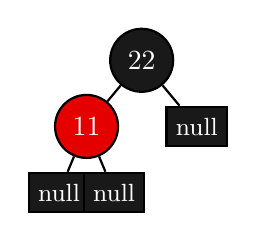
\begin{tikzpicture}[
          scale=0.7,
          red_node/.style={circle, draw, thick, fill=red!90!black, text=white, minimum size=0.8cm},
          black_node/.style={circle, draw, thick, fill=black!90, text=white, minimum size=0.8cm},
          null_node/.style={rectangle, draw, thick, fill=black!90, text=white, minimum size=0.5cm, font=\small},
          edge/.style={draw, thick, -}
        ]
        % Third tree (valid red-black tree)
        % Nodes
        \node[black_node] (n22) at (0,0) {22};
        \node[red_node] (n11) at (-1,-1.2) {11};
        \node[null_node] (n22r) at (1,-1.2) {null};
        \node[null_node] (n11l) at (-1.5,-2.4) {null};
        \node[null_node] (n11r) at (-0.5,-2.4) {null};
        
        % Edges
        \draw[edge] (n22) -- (n11);
        \draw[edge] (n22) -- (n22r);
        \draw[edge] (n11) -- (n11l);
        \draw[edge] (n11) -- (n11r);
        \end{tikzpicture}
        \caption{Valid: Root is black, red nodes have no red children, and all paths from node to null leaves have the same number of black nodes.}
        \label{fig:rb-valid}
      \end{subfigure}
      \caption{Examples and non-examples of red-black trees.}
      \label{fig:red-black-tree-examples}
    \end{figure}

    Remember that red black trees are also just binary search trees, and so some of the operations are the same.  
    \begin{enumerate}
      \item contains (search) method is the exact same thing as BST 
      \item The add method needs to be slightly modified, since after we add, we need to make sure that the resulting tree is a red-black tree. This is done in three steps: 
      \begin{enumerate}
        \item Run the regular BST add 
        \item Color the new node red 
        \item Fix the tree to reestablish red-black tree properties. This is extremely complicated with different cases, but it all essentially uses some sort of recoloring and a (right or left) rotation of the tree. 
      \end{enumerate}
    \end{enumerate}
  \end{definition}

  Note that there are binary search trees that cannot be turned into a red-black tree. 
  \begin{center}
    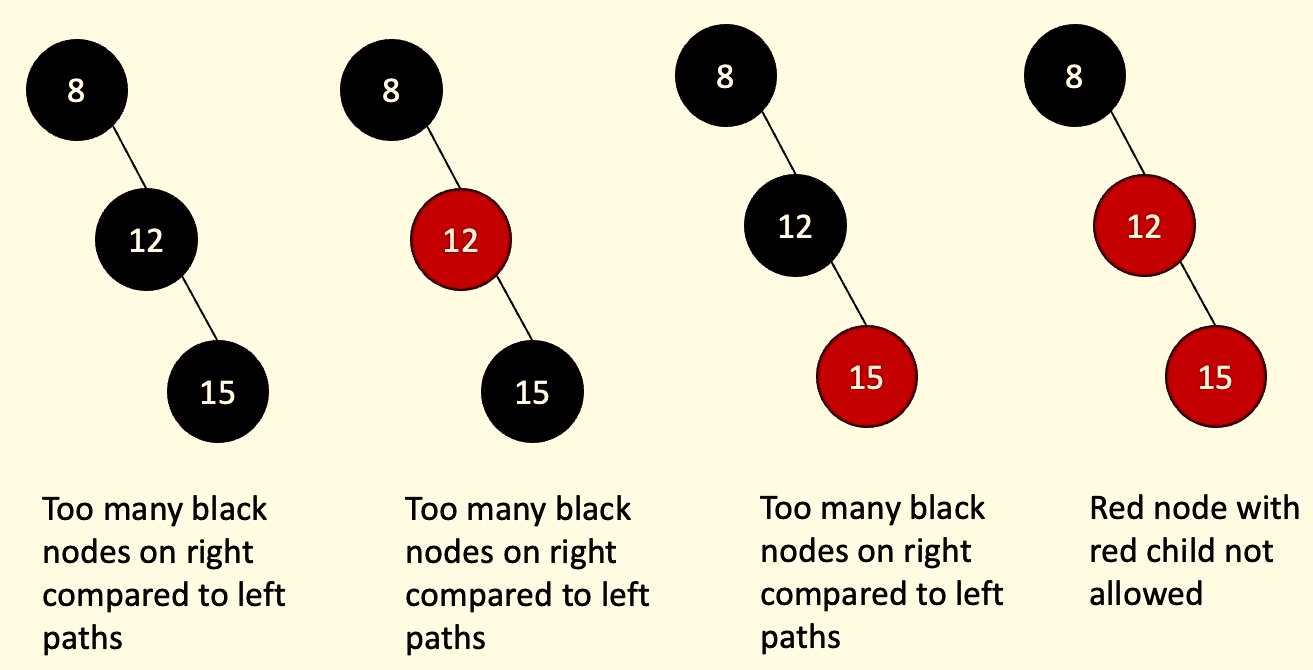
\includegraphics[scale=0.3]{img/impossible_red_black.png}
  \end{center}

  This is intentional because red-black tree properties guarantee approximate balance. If we can turn a binary search tree into a red-black tree, then it logically follows that the original BST was approximately balanced. Note that a red black tree does not make searching asymptotically faster in any way; it just takes care of the worst-case. 

\subsection{Tries}

